\chapter{Introduction} \label{intro}
Trust and confidence that a system will behave as expected is stress-tested every day, whether from operational issues (expected or unexpected), environmental impacts and system hazards
or malicious unauthorized parties. Confidence and trust require organized attention to the key characteristics of a system and the collection of appropriate evidence that the desired characteristics are being achieved.

Medical software is one of the domains that is difficult to prove its trustworthiness; the implementation details are very sensitive thus it might not be open-sourced to let every user to verify the program themself, but without knowing the implementation details, it is challenging to gain confidence and trust especially over the medical software. The medical software can be used to examine the human bodies, inject medicine to the patients, saving the patients life. On the other hand, a very small implementation mistake could cause people's life.

Under this context, we want to explore the feasibility of applying assurance cases over a medical software from the beginning of the development. With selected arguments and evidences, we want to show to the domain experts that the software delivers correct outputs when used for its intented use/purpose in its intended environment, and within its assumed operating assumptions.


\section{Objective} \label{obj}
In this study, we present the result of applying of assurance cases in a developing medical software to build the stakeholders' confidence in this software. The software AortaGeomRecon is a 3D Slicer extension module aims to semi-automatically build 3D geometry of the Aorta from the patient's chest ct scans. Assurance cases are a method for providing assurance for a system by giving an
argument to justify a claim about the system, based on evidence about its design, development, and tested behavior. This case study first presents the problem of Organ/Aorta Segmentation, and the existing solutions which might take time and efforts from the domain experts. Then, we present our algorithm's workflow and logic, and the work environment of using this module in 3D Slicer. Finally, we discussed our assurance cases with selected arguments and evidence, to explain why with these selected pieces, we were able to build confidence in the medical software.

\section{Background} \label{bg}
Aorta is the largest artery that carries blood from the heart to the circulatory system. It has a cane-liked shape with Ascending aorta, Aortic arch and Descending aorta. 

\begin{figure}[H]
    \centering
    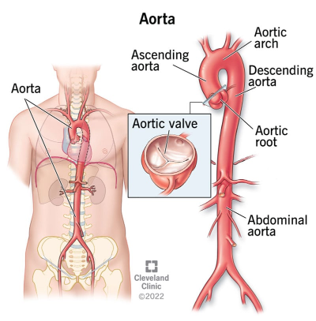
\includegraphics[width=0.7\textwidth]{figures/Sample/Aorta.png}
    \caption[Aorta]{Aorta}
    \label{fig_aorta}
\end{figure}

Aorta segmentation in CT scans is important for:
\begin{itemize}
\item Coarctation of the aorta
\item Aortic calcification quantification
\item To guide the segmentation of other central vessels. 
\end{itemize} ~\\

\section{Thesis Outline} \label{TO}

The thesis is organized into three broad parts. In chapter 2, we introduce our program \progname{} by mentioning the existing methods, the AortaGeomRecon's algorithm overview and step by step  workflow. We explain necessary terms and information to understand how the software functionsfinally, and the 3D Slicer extension module that the user interacts with to get the segmentation result with our algorithm. In chapter 3, we present our assurance case, some sections of our SRS, Design Documents, Module Guide, Algorithm Review, and a test case we developed for verifying and validating the correctness of program \progname{}. Finally, future work is proposed and conclusions are drawn based on the developed assurance case, SRS, segmentation algorithm and 3D Slicer module extension.